\chapter{Introduction and Background}
\label{ch: intro}

\graphicspath{{Figures/Intro/}{./}} 

Quantiles are the cutting points of a statistical distribution by its ranking. Specifically, the $\tau$-quantile is the cutting point that divides the distribution by probability $\tau$. Let $\tau$-q denotes the $\tau$-quantile. For example, a $0.5$-q is the median of a distribution, such that there is a $50\%$ probability that a random sample is smaller than it.
The quantiles are an important statistical feature of distributions for their values roughly reflects the density of the distribution.
For example, Fig \ref{fig: quant_example} shows the two intervals between [$0.5$-q, $0.9$-q] and [$0.9$-q, $0.99$-q] has similar value, while the former contains 40\% data and the latter contains only 9\% data. Without any other information, this alone leads to the implication that the distribution is denser in the former interval than the latter.

\begin{figure*}[h!]
    \centering
	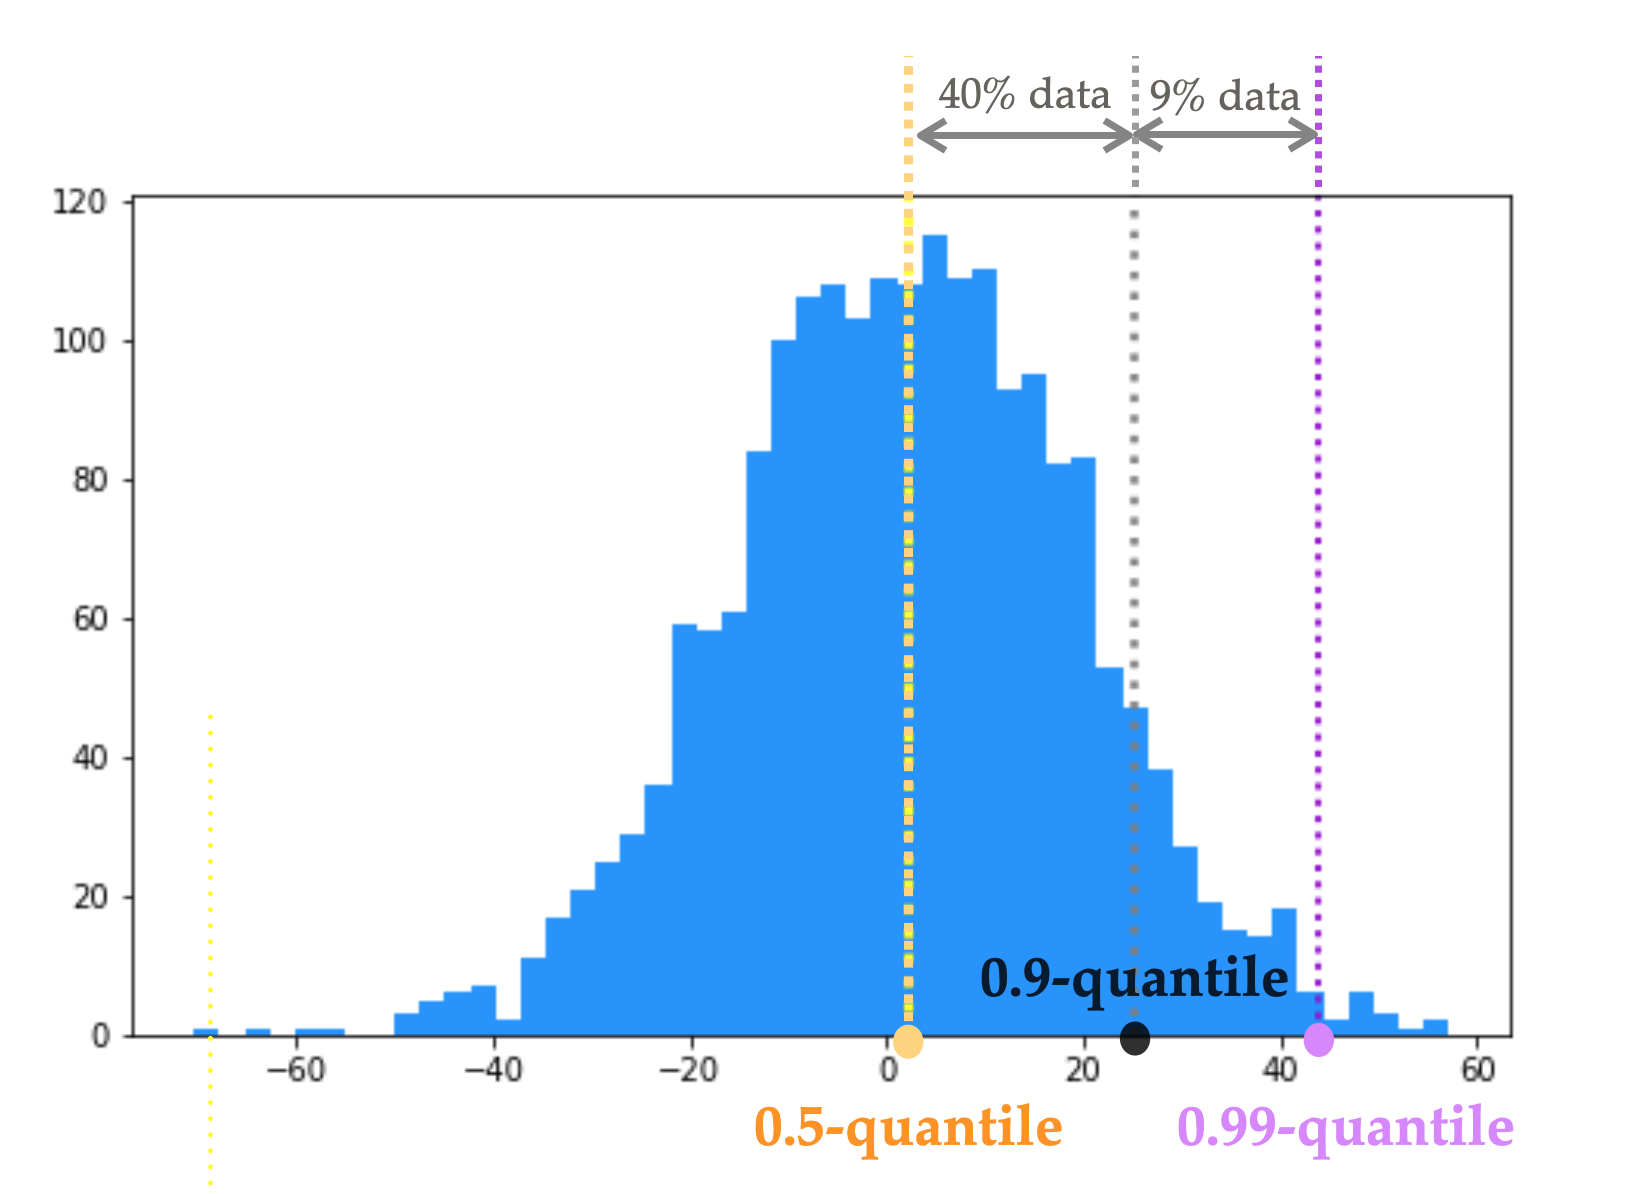
\includegraphics[width=0.6\columnwidth]{quant_example.png}
    \caption{Quantiles (0.5-q, 0.9-q and 0.99-q) of a dataset containing 2000 random samples from a Gaussian distribution (mean = 2, standard deviation = 18)}
    \label{fig: quant_example}
\end{figure*}

The aaaaa

Batch algorithm/True quantile: the naive sorting

Quantile estimation on data streams

Gradient descent and SGD (insert picture) introduce in short paragraphs

Fig \ref{fig: structure} shows the layout of the contents of the thesis.

\begin{figure*}[h!]
    \centering
	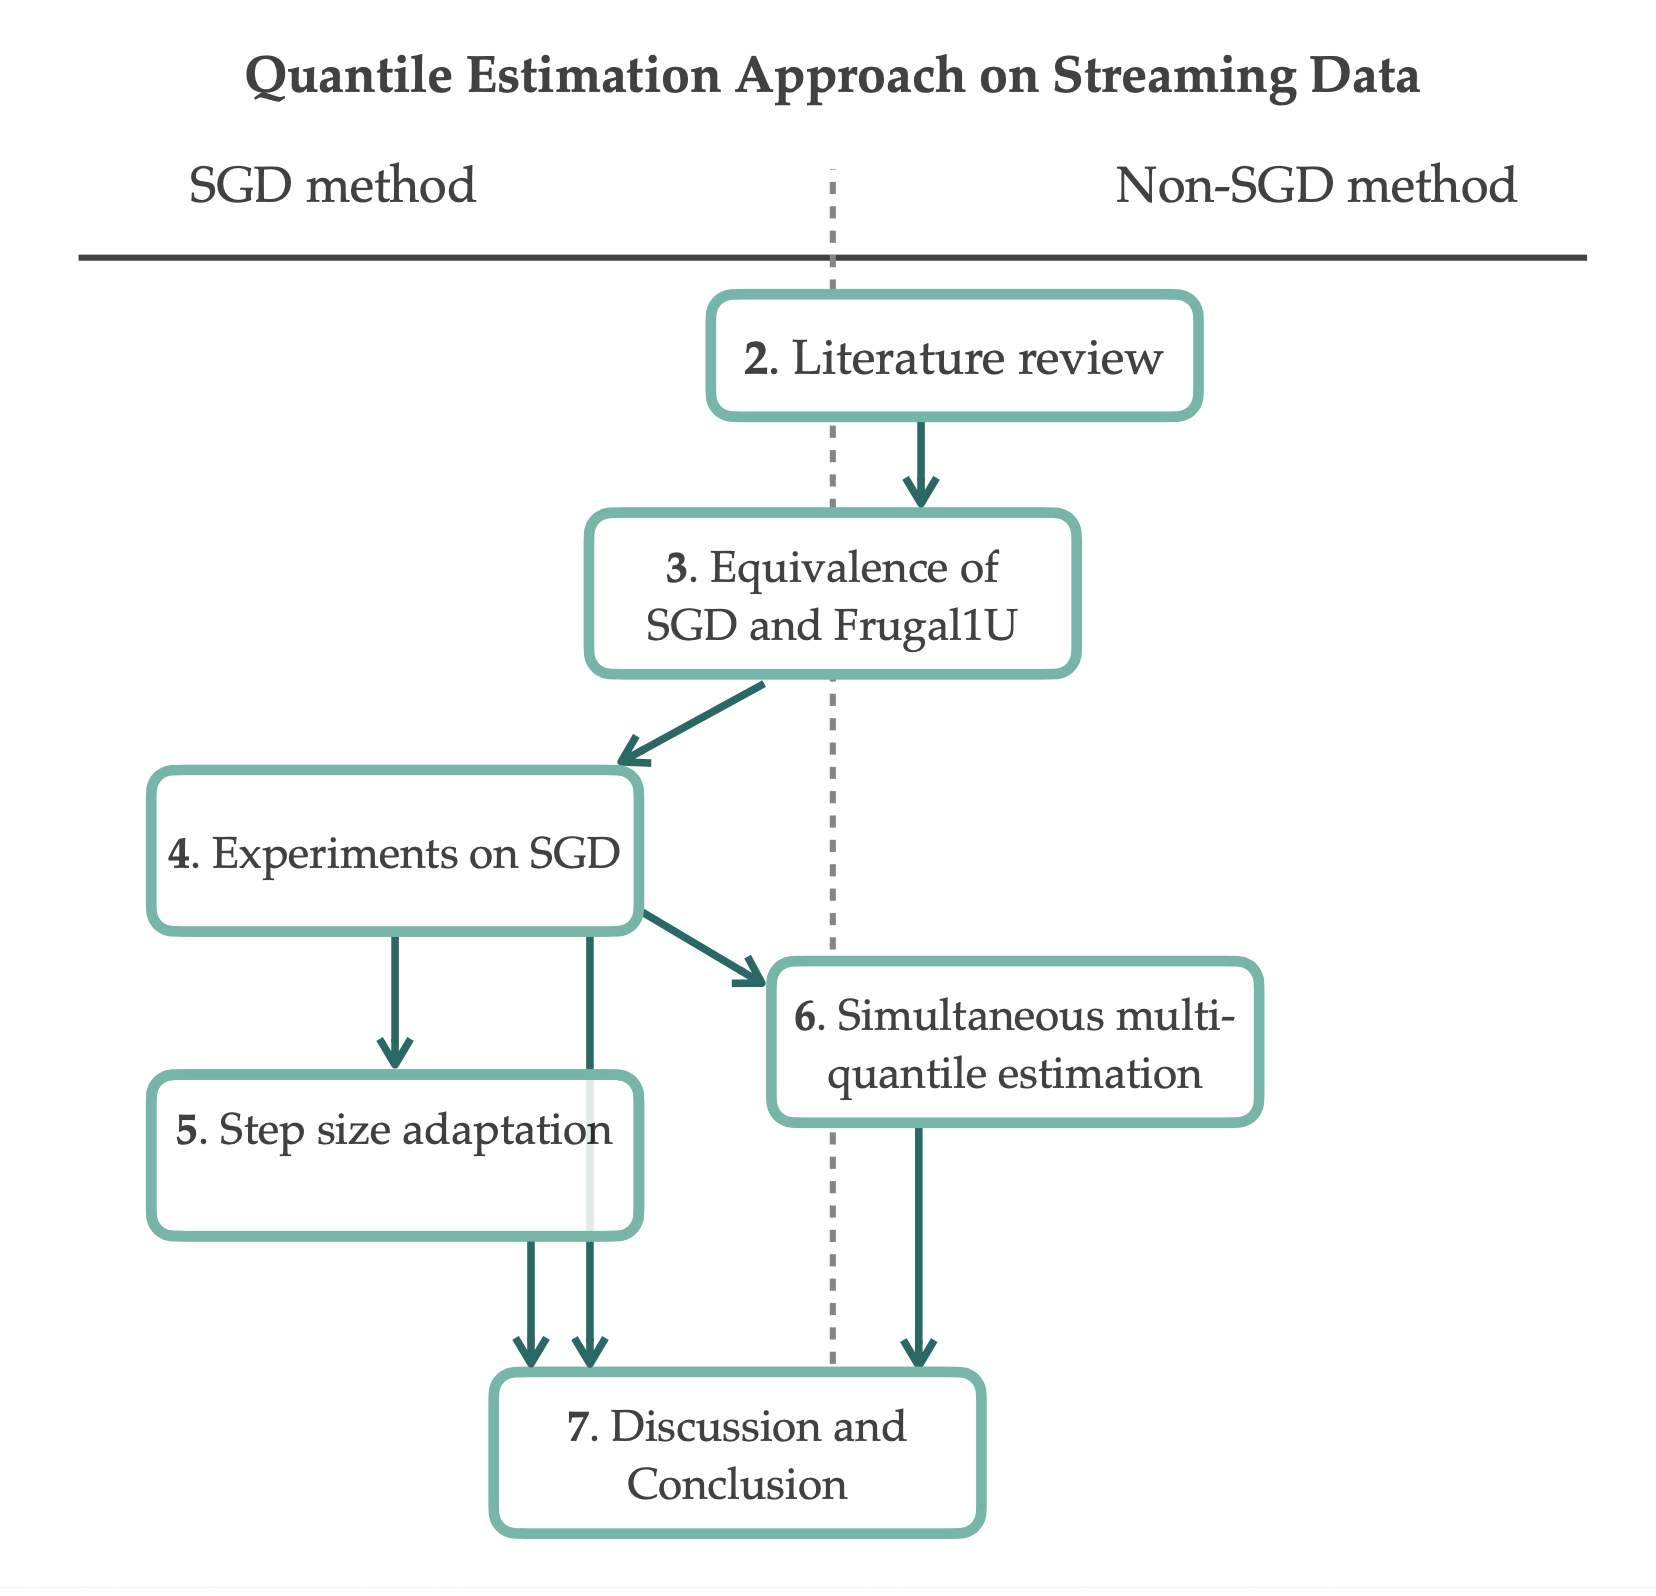
\includegraphics[width=0.6\columnwidth]{structure.png}
    \caption{The relationship between topics covered in the thesis}
    \label{fig: structure}
\end{figure*}